\chapter{Hiện Thực Hệ Thống Luyện Nghe Tiếng Anh}

\ifpdf
    \graphicspath{{Chapter4/Chapter4Figs/PNG/}{Chapter4/Chapter4Figs/PDF/}{Chapter4/Chapter4Figs/}}
\else
    \graphicspath{{Chapter4/Chapter4Figs/EPS/}{Chapter4/Chapter4Figs/}}
\fi

\section{Thiết kế lớp giao diện ứng dụng}

Các lớp giao diện được thiết kế tách rời nhằm đảm bảo tính thuận tiện và trực quan nhất cho ứng dụng.

\begin{figure}[!htb] 
\centering
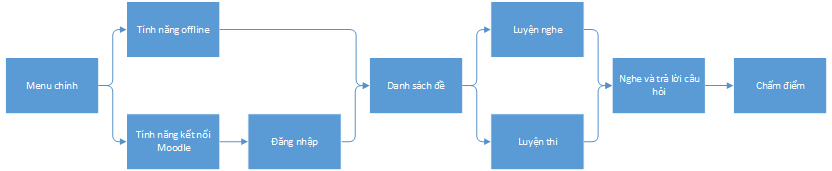
\includegraphics[width=0.9\textwidth]{gui.png}
\caption{Sơ đồ thiết kế giao diện chương trình}
\end{figure}

Sau khi lựa chọn tính năng chương trình, danh sách các đề sẽ được hiển thị cho người dùng chọn. 

Và sau khi đã chọn được một đề, cửa sổ chọn hình thức làm bài sẽ được xổ ra. 

Người dùng sẽ chọn hình thức luyện nghe hay luyện thi với tính năng bị hạn chế hơn. 

Giao diện làm bài hỗ trợ duyệt tới lui giữa các câu hỏi và duyệt nhanh giữa những câu còn chưa trả lời. 

Sau khi làm bài, phần chấm điểm sẽ hiển thị điểm số cùng các kỹ năng của người dùng. 

Sau đó là các kết quả làm bài ở những lần trước dưới dạng đồ thị để người dùng theo dõi quá trình ôn luyện của mình.

\section{Hiện thực tính năng luyện nghe offline}

Khi không có kết nối Internet, ứng dụng vẫn có thể hoạt động được nhờ việc sử dụng các dữ liệu mẫu đã được lưu trong chương trình dưới dạng XML. Người sử dụng vẫn có thể thực hiện các chức năng làm bài, chấm bài và xem kết quả một cách bình thường.

\begin{figure}[!htb] 
\centering
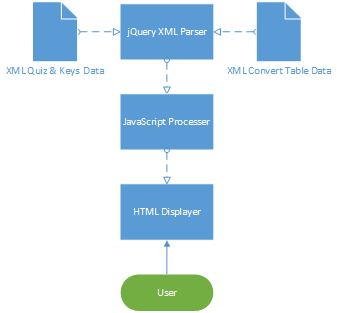
\includegraphics[width=0.5\textwidth]{offline.png}
\caption{Sơ đồ xử lý của các thành phần phía client tương ứng với chức năng nghe offline}
\end{figure}

Các bước hoạt động:

\quad - Mặc định, ứng dụng sẽ kiểm tra danh sách các đề có sẵn trong bộ nhớ. Sau khi người dùng chọn đề, nội dung các câu hỏi trong đề sẽ được hiển thị lần lượt lên màn hình, đồng thời nội dung audio cũng được chạy và bắt đầu tính thời gian làm bài.

\quad - Các câu trả lời của người dùng sẽ được lưu tạm vào SessionStorage, và sau khi có lệnh nộp bài, nội dung trong biến này sẽ được so sánh với các đáp án của đề tương ứng theo từng phần tử của mảng.

\quad - Chênh lệch nội dung của 2 mảng sẽ cho biết kết quả bài làm của người dùng. Kết quả này sẽ được lưu lại để làm thống kê về sau.


\section{Hiện thực tính năng kết nối với Moodle}
\subsection{Cấu trúc tương tác giữa client và server}

\begin{figure}[!htb] 
\centering
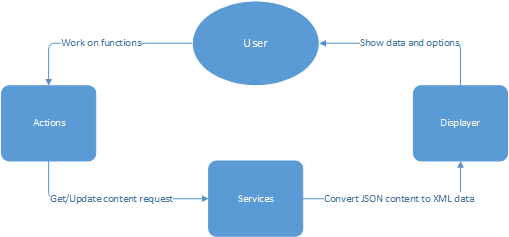
\includegraphics[width=0.8\textwidth]{server-client.png}
\caption{Sơ đồ cấu trúc ứng dụng ở cả server và client}
\end{figure}

Trong đó, chức năng cụ thể của từng khối như sau:

\quad - Actions: các thành phần JavaScript tập trung xử lý các tương tác của người dùng và chịu trách nhiệm trong việc gửi nhận dữ liệu.

\quad - Services: các dịch vụ của server Moodle giúp việc quản lý khóa học và đảm nhiệm việc cung cấp nội dung cho phía client.

\quad - Displayer: các thành phần HTML đảm nhiệm việc hiển thị thông tin về người dùng, khóa học và nội dung đề thi một cách trực quan và sinh động tới người dùng.

\subsection{Cấu hình trên moodle}

Trước hết ta phải ta phải đăng nhập vào Moodle với quyền admin.

Ta kích hoạt web service:

\quad - Vào Access Settings > Site administration > Advanced features
 
\quad - Chọn 'Enable web services' rồi chọn 'Save Changes'

Tạo web service:

\quad - Vào Access Settings > Site administration > Plugins > Web services > External services

\quad - Chọn Add new custom service

\quad - 'Authorised users only' - Nếu chọn, thì ta phải tự thêm vào các user được phép truy cập.
 
\quad - Gõ tên web service và chọn Enabled.

\quad - Click 'Add service'.

\begin{figure}[!htb] 
\centering
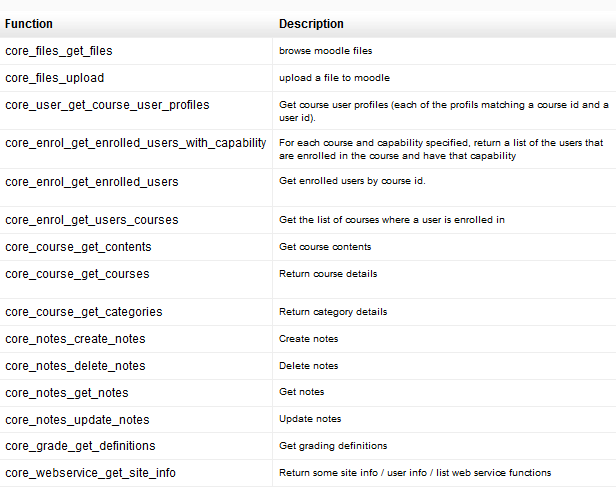
\includegraphics[width=0.8\textwidth]{wsfunction.png}
\caption{Một số web services cần dùng trong ứng dụng}
\end{figure}

Thêm các hàm cần sử dụng vào web service:

\quad - Chọn 'Add functions' link

\quad - Chọn các hàm cần sử dụng và click vào 'Add functions'

Để có thể gọi web sevice được ta cần phải truy cập vào cơ sở dữ liệu của Moodle, tìm đến table có tên là "mdl\_external\_services", thêm vào cột shortname tên web services.

\begin{figure}[!htb] 
\centering
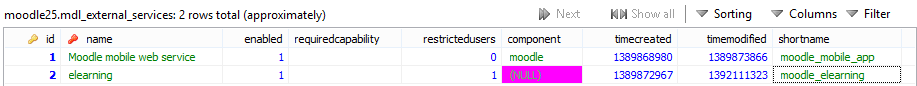
\includegraphics[width=0.8\textwidth]{addShortNameWS.png}
\caption{Cách thêm shortname cho web service}
\end{figure}
 
Bên cạnh sử dụng các hàm có sẵn của Moodle, ta cũng có thể tự tạo ra web service với các hàm do ta tự cài đặt nếu các hàm có sẵn không đáp ứng được nhu cầu.

\subsection{Mô hình xử lý trên client}

Client khi kết nối tới Moodle cũng có cơ chế làm việc tượng tự với khi đọc và xử lý dữ liệu offline. Nhưng nhờ kết nối tới máy chủ nên lượng dữ liệu sẽ phong phú và mang tính linh động cao hơn.

\begin{figure}[!htb] 
\centering
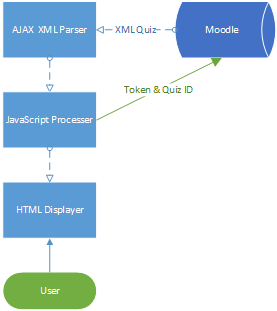
\includegraphics[width=0.5\textwidth]{client-onl.png}
\caption{Sơ đồ xử lý của các thành phần phía client tương ứng với chức năng luyện nghe có kết nối tới Moodle}
\end{figure}

Trong mục này, nhóm chúng em muốn giới thiệu về cách gọi các service của Moodle và cách xử lý dữ liệu trả về từ máy chủ trên client.

Để ứng dụng có thể tương tác với Moodle thì việc gửi và nhận dữ liệu đều liên quan đến một tham số là user token. Đó là một chuỗi ký tự đã được mã hóa, đặc trưng cho từng người sử dụng để xác thực phiên làm việc và quyền truy xuất đến service. Và để có được chuỗi token này, khi người sử dụng tiến hành đăng nhập ứng dụng phải gọi một HTTP request tới service cấp token với các tham số gồm username, password và tên của service.

Ta có ví dụ sau: \url{http://127.0.0.1/moodle25/login/token.php?username=09520266\&password=1qaz@WSX&service=moodle_elearning} sẽ đăng nhập với tên đăng nhập là “09520266” và mật khẩu là “1qaz@WSX”. Nếu đăng nhập thành công, server sẽ trả về chuỗi token ứng với phiên đăng nhập: 

“token: 247bc66c021e11f2e888f2476d71a44d” ứng với user "09520266".

Sau khi đã có chuỗi token, với mỗi lời gọi tới service cần phải đính chuỗi token đã lấy được như một tham số. Mỗi request sẽ có 2 phần chính:

\quad - Path: chứa đường dẫn của service

\quad - Query: chứa chuỗi token xác thực và các tham số cần thiết để lấy dữ liệu. Các tham số cách nhau bởi dấu “\&”.

Ví dụ: lời gọi \url{http://127.0.0.1/moodle25/webservice/rest/server.php?wsfunction=core_course_get_courses&wstoken=247bc66c021e11f2e888f2476d71a44d} sẽ gọi tới service “core\_course\_get\_courses” nhằm lấy về danh sách các khóa học của hệ thống. 

Trong đó, phần Path là \url{http://127.0.0.1/moodle25/webservice/rest/server.php} và phần Query có 2 tham số là “wsfunction=core\_course\_get\_courses” và “wstoken=247bc66c021e11f2e888f2476d71a44d”.

Như vậy, khi ghép tham số “wsfunction” với tên các service đã liệt kê bên trên, ta được một lời yêu cầu tới máy chủ Moodle để gọi service tương ứng và nhận dữ liệu XML với các thành phần key-value mà máy chủ trả về.


\section{Hiện thực việc triển khai ứng dụng}
Một số hình ảnh thực tế của ứng dụng mà nhóm khóa luận đã thực hiện được:

\begin{figure}[!htb] 
\centering
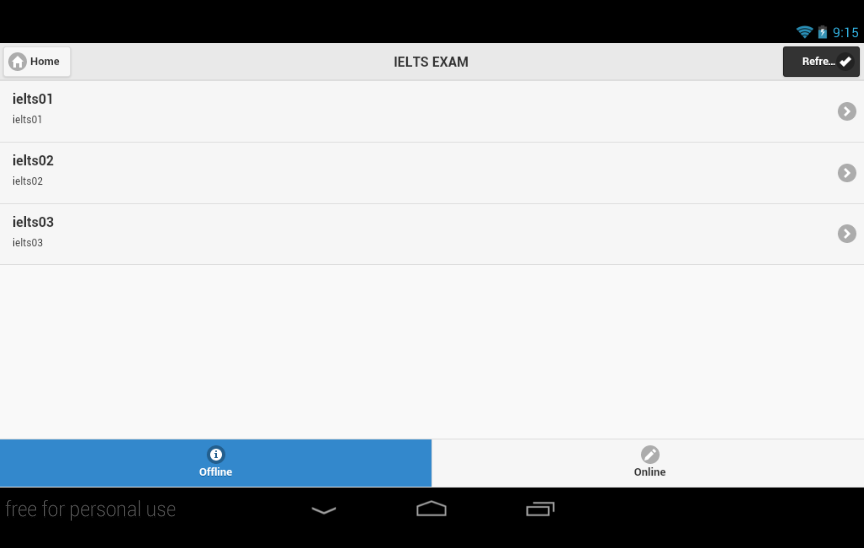
\includegraphics[width=0.8\textwidth]{1list_screen.png}
\caption{Màn hình danh sách các bài luyện nghe offline}
\end{figure}

\newpage

\begin{figure}[!htb] 
\centering
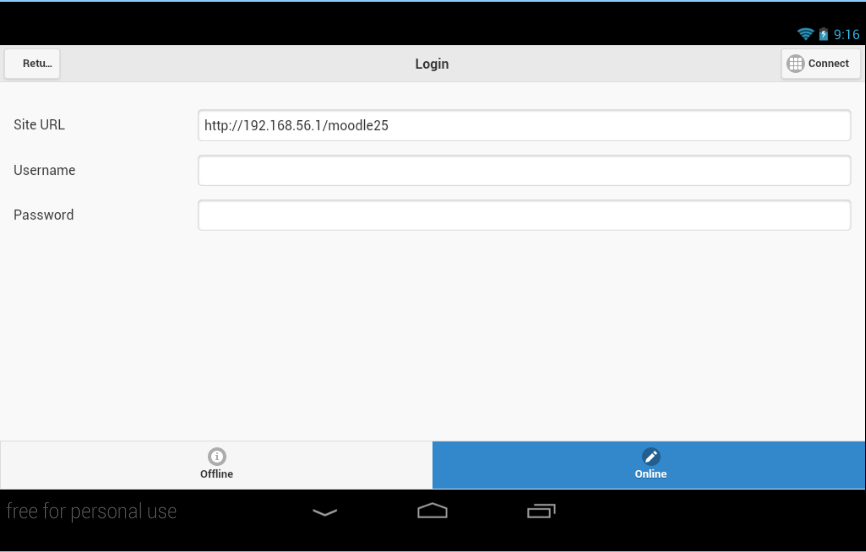
\includegraphics[width=0.8\textwidth]{2login_screen.png}
\caption{Màn hình đăng nhập vào Moodle}
\end{figure}

\begin{figure}[!htb] 
\centering
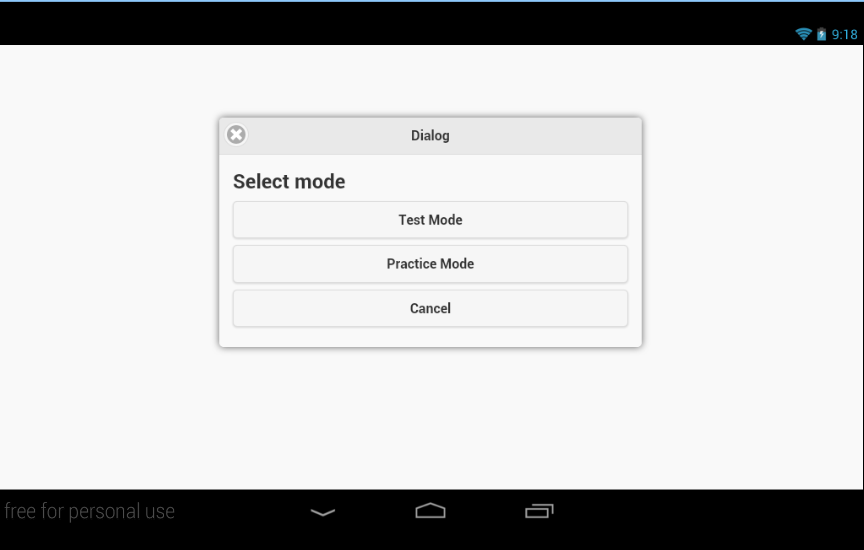
\includegraphics[width=0.8\textwidth]{3select_mode.png}
\caption{Màn hình chọn chế độ}
\end{figure}

\newpage

\begin{figure}[!htb] 
\centering
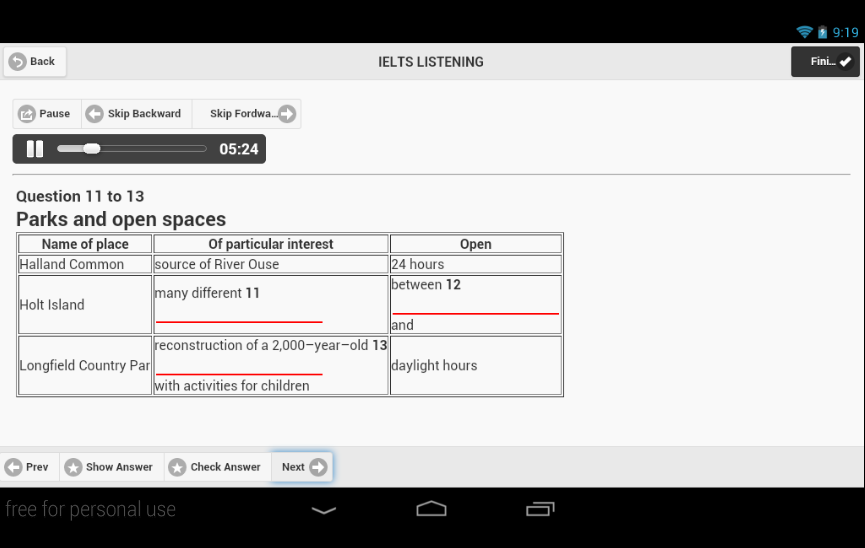
\includegraphics[width=0.8\textwidth]{4pracmode_1.png}
\caption{Màn hình làm bài với dạng câu hỏi điền từ}
\end{figure}

\begin{figure}[!htb] 
\centering
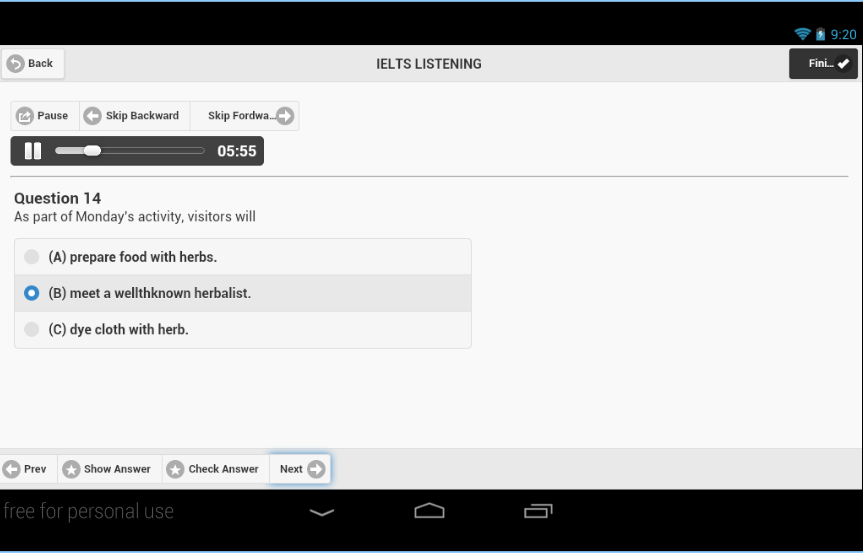
\includegraphics[width=0.8\textwidth]{5pracmode_2.png}
\caption{Màn hình làm bài với dạng câu hỏi trắc nghiệm}
\end{figure}

\newpage

\begin{figure}[!htb] 
\centering
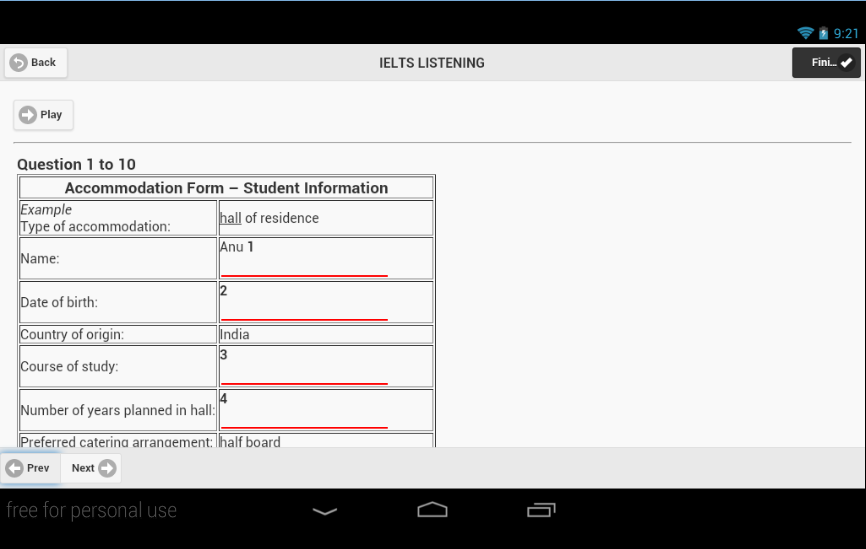
\includegraphics[width=0.8\textwidth]{6testmode.png}
\caption{Màn hình chức năng luyện nghe ở chế độ thi thử}
\end{figure}

\begin{figure}[!htb] 
\centering
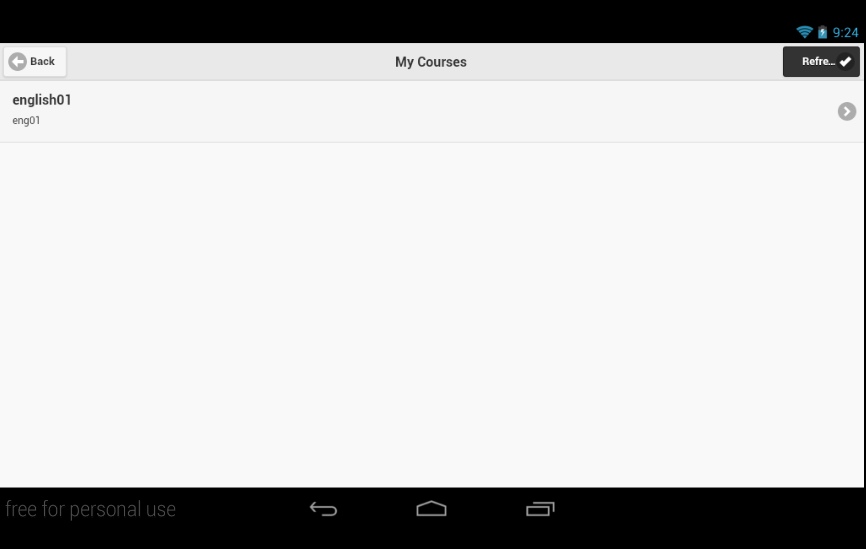
\includegraphics[width=0.8\textwidth]{7listcourse.png}
\caption{Màn hình danh sách khóa học có trên Moodle}
\end{figure}

\newpage

\begin{figure}[!htb] 
\centering
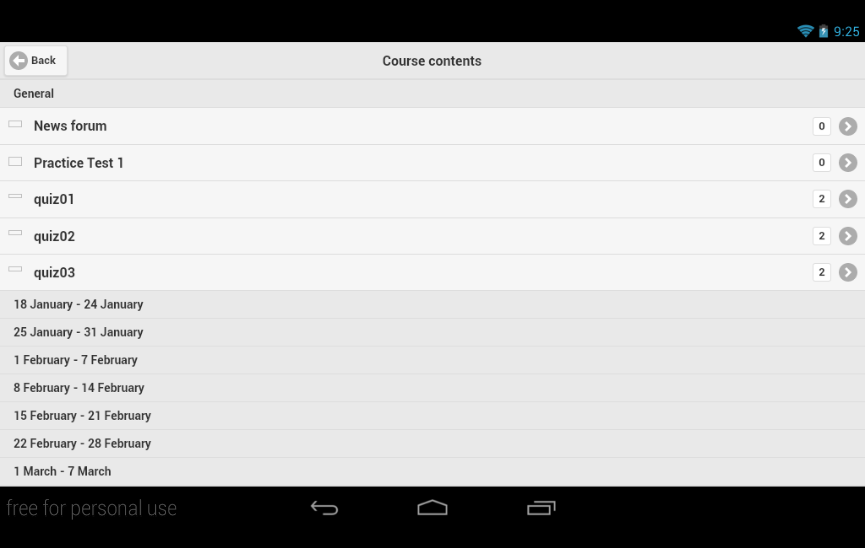
\includegraphics[width=0.8\textwidth]{8coursecontent.png}
\caption{Màn hình nội dung khóa học - liệt kê các bài nghe do giáo viên soạn}
\end{figure}

\begin{figure}[!htb] 
\centering
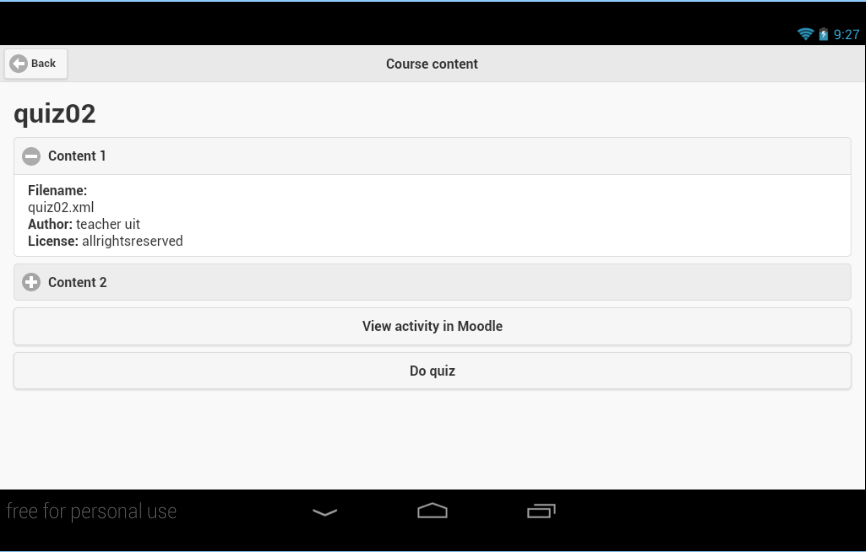
\includegraphics[width=0.8\textwidth]{9quizcontent.png}
\caption{Màn hình nội dung một bài luyện nghe - Nhấn nút "Do quiz" để luyện tập}
\end{figure}

\newpage

\section{Tổng kết chương}

Trải qua bốn chương mà chúng em trình bày, khóa luận đã nghiên cứu và xây dựng được chương trình luyện nghe tiếng Anh theo cấu trúc đề thi IELTS trên máy tính bảng, hỗ trợ hai chức năng chính đó là luyện nghe offline không cần đến Internet, luyện nghe online thông qua kết nối đến Moodle.

Điểm nổi bật của ứng dụng mà chúng em xây dựng so với các ứng dụng tương tự khác, đó là:

\quad - Khả năng chạy được trên nhiều nền tảng di động khác nhau như iPhone, iPad, Android, Windows Phone,...

\quad - Tính năng kết nối đến Moodle tạo nên sự phong phú về nội dung bài học.

Bên cạnh đạt được những kết quả tốt đẹp, khóa luận cũng còn mắc phải một số hạn chế. Chúng em xin được phép trình bày rõ về những hạn chế, khó khăn trong chương cuối cùng - kết luận và hướng phát triển.